\subsection[LBS Definitionen]{LBS Definitionen
 \\ \textnormal{\small{\textit {Verfasst von Patrick Senneka}}}}

%\textbf{Bedeutung für Firmen, NSA, Privatpersonen, verbreitete Apps}

%Bedeutung für: Konzerne, Werbeindustrie, NSA, IT-Forensik \linebreak
%Privatpersonen: Schnellste Zugverbindung, Restaurant, Freunde treffen, Reiseführer


%\textbf{Definitionen}

Für diese Arbeit über Location-based Services ist es wichtig zu definieren, was unter diesem Begriff genau zu verstehen ist. Der erste Schritt dazu ist den Begriff ins deutsche zu übersetzen. Unter Location-based Services versteht man nach einer wörtlichen Übersetzung Standort-bezogene Dienste. Nach der deutschen Sprache wäre nun anzunehmen, dass es Dienste sind, die unter Zuhilfenahme des Standorts angeboten werden. In der Literatur gibt es allerdings nicht eine feste Definition, die mit dem ersten Location-based Service festgelegt wurde. Es ist vielmehr so, dass es mehrere Begrifflichkeiten gibt, die nicht das gleiche aussagen, aber dennoch so verwendet werden. Vergleiche hierzu Zitat 1.1 von Alex Küpper.

\begin{table}[h]
	\centering
	\begin{tabular}{|p{16cm}|}\hline
		\textbf{Zitat 1.1:} \glqq Although Location-based Services (LBSs) have been an issue in the field of mobile communication for many years, there exists neither a commen definition nor a commen terminology for them. For example, the terms location-based service, location-aware service, location-related service, and location service are often interchangeably used. \cite[S.1]{Kuepper2005} \\ \hline
		\textbf{Übersetzung:} Obwohl Location-based Services (LBSs) schon seit vielen Jahren ein Thema sind, existiert weder eine einheitliche Definition noch eine einheitliche Begrifflichkeit. Zum Beispiel werden die Ausdrücke lacation-baded service, location-aware service, location-related service and location service oft austauschbar verwendet. \\ \hline
	\end{tabular}
\end{table}


Eine eindeutige Definition zu Location-based Services wurde von Jochen Schiller in seinem Buch \glqq Location-Based Services \grqq aufgestellt. Vergleiche Definition 1.2.

\begin{table}[h]
	\centering
	\begin{tabular}{|p{16cm}|}\hline
		\textbf{Definition 1.2:} \glqq The term location-based services (LBS) is a recent concept that denotes applications integrating geographic location (i.e., spatial coordinates) with the general notion of services. \grqq \cite[S.1]{Schiller2004}\\ \hline
		\textbf{Übersetzung:} Der Begriff Location-based Services (LBS) ist ein aktuelles Konzept, dass Applikationen, die geografische Standorte integrieren (z.B., räumliche Koordinaten) mit dem eigentlichen Gedanken eines Services vereint. \\ \hline
	\end{tabular}
\end{table}

Obwohl die Definition für Location-based Services von Jochen Schniller klar und eindeutig erscheint, besteht nach der Aussage von Alex Küpper noch Klärungsbedarf bezüglich der andren oft synonym verwendeten Begriffen:
\begin{itemize}
\item location service
\item location-based service
\item location-aware service
\item and location-related service
\end{itemize}



\textbf{location service} \\
Der Hauptunterschied zwischen Location Service und Location-based Services besteht in der Verarbeitung der Standortdaten. Bei einem Location Service wird der Standort eines Objekts (z.B eines Handys) bestimmt. Dieser ermittelte Standort wird dann als Service extern bereitgestellt. Die Standortdaten werden also erfasst und zur Verfügung gestellt, ohne diese zu verarbeiten.
Der Unterschied zu einem Location-based Service besteht darin, dass bei diesem die Standortdaten weiterverarbeitet werden. Ein location service ist also einer der wichtigsten Bestandteile eines Location-based Service, der dabei die Standortdaten nicht extern bereitstellt, sondern zu Weiterverarbeitung einem Location-based Service zu Verfügung stellt.
\cite[S.1-2]{Kuepper2005}

\textbf{location-based service} \\
Entspricht der Definition 1.2 nach Schiller.


\textbf{location-aware service} \\
\begin{table}[h]
	\centering
	\begin{tabular}{|p{16cm}|}\hline
		\textbf{Definition 1.3:} \glqq Generally, context-aware services are defined to be services that automatically adapt their behavior, for example, filtering or presenting information, to one or several parameters reflecting the context of a target. These parameters are termed context information.\grqq \cite[S.2]{Kuepper2005}\\ \hline
		\textbf{Übersetzung:} Im Allgemeinen sind context-aware services als solche definiert, dass sie automatisch ihr Verhalten, z.B. filtern oder darstellen von Informationen, an ein oder mehrere Parameter anpassen, die den Kontext des Ergebnisses widerspiegeln. Diese Parameter werden als Kontext Informationen bezeichnet. \\ \hline
	\end{tabular}
\end{table}

Die in Definition 1.3 beschriebene Kontext Parameter können einerseits Daten sein, die direkt von einem Sensor wie zum Beispiel einem Thermometer oder Positionssensor sein. Diese Rohdaten bilden den Primären Kontext. Andererseits gibt es noch aus Rohdaten abgeleitete Kontextdaten. Diese entstehen durch Kombination und oder Filterung von Rohdaten. Das sind die Sekundär Kontextdaten. 
\cite[S.2]{Kuepper2005}

Die beispielhafte Aufzählung von Rohdaten zeigt, dass context-aware services location-aware services mit einschließen könne allerdings nicht müssen. Verdeutlicht wird das durch Abbildung \ref{fig:context-aware services}.


\begin{figure}[h]
\centering
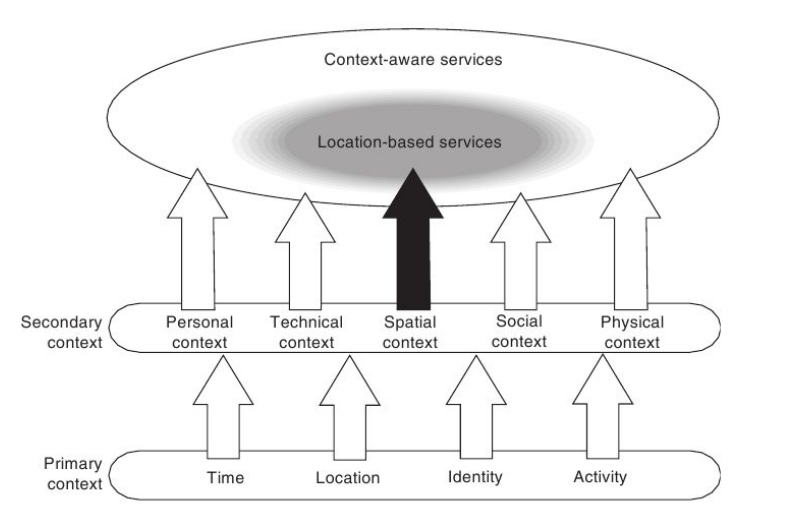
\includegraphics[width=0.99\textwidth]{ref/images/definitionK.png}
\caption[Context-aware services]{Context-aware services}
\label{fig:context-aware services}
\cite[S. 2]{Kuepper2005}
\end{figure}

\newpage
\textbf{location-related service} 

Location-related service ist ein noch breiter gefasster Begriff, als Location-aware service. Es ist als mobiler Service definiert, bei welchem Standorte eine große Bedeutung spielen. Vergleiche hierzu Definition 1.4.

\begin{table}[h]
	\centering
	\begin{tabular}{|p{16cm}|}\hline
		\textbf{Definition 1.4:} \glqq Therefore, mobile services relying on this importance of location will be referred to in the following as locationrelated services (LRS). Location Based Services (LBS) are a sub-category of LRS \grqq \cite[S.5]{strueker2003}\\ \hline
		\textbf{Übersetzung:} Mobile Services, die sich auf die Bedeutung von Standorten beziehen werden im folgenden als locationrelated services (LRS) referenziert. Location Based Services (LBS) sind eine Unterkategorie von LRS  \\ \hline
	\end{tabular}
\end{table}





